\chapter{Observabilidade}

Com o aumento da complexidade do projeto, é importante saber quando algum usuário teve problemas ao 
tentar acessar alguma rota que não funcionou corretamente.

O NGINX possui um arquivo de logs localizado em \verb|/var/log/nginx/access.log|. No entanto, com o 
aumento do número de acessos, esse arquivo se torna cada vez mais difícil de interpretar.

A solução é utilizar uma ferramenta que processe esse arquivo de log e exiba os dados em uma 
interface gráfica. Para isso, usei o GoAccess \cite{goaccess}. Ele é um programa para Linux que, 
ao receber o arquivo de log, gera um arquivo HTML como saída.

\lstinputlisting[label=cod
, title={GoAccess}, caption={Comando para executar o GoAccess}, language=bash]{code/goaccess.sh}

Observe que o arquivo de log que estou acessando é \verb|/var/log/nginx/nginx-access.log|. Isso foi 
necessário porque a imagem Docker do NGINX que uso por padrão cria um link simbólico de \verb|/var/log/nginx/access.log| 
para \verb|/dev/stdout|, o que impossibilitava o acesso ao arquivo. Para contornar esse problema, 
precisei configurar o arquivo de configuração do NGINX para que os logs de acesso fossem gravados e
m outro local.

Também é importante destacar que o GoAccess não serve o arquivo HTML gerado automaticamente, apenas 
o cria. A minha solução foi utilizar o próprio NGINX para servir esse arquivo na rota \texttt{a4barros.com/private/report}. 
Essa URL está protegida por autenticação HTTP básica. O arquivo HTML gerado é estático e não é 
atualizado automaticamente. Existe, contudo, a opção de usar o parâmetro \texttt{--real-time-html}, 
que abre um socket na porta 7890 e adiciona um código JavaScript à página HTML para atualizações em 
tempo real. No entanto, como não queria manter essa porta aberta, optei por criar um script shell 
que recria essa página a cada 3 minutos.

\lstinputlisting[label=cod
, title={GoAccess}, caption={Comando para executar o GoAccess a cada 3 minutos}, language=bash]{code/goaccess.Dockerfile}

Em média, o GoAccess consegue processar 101.245,3 linhas de log por segundo \cite{goaccess-speed},
então rodar ele a cada três minutos para a quantidade de acessos que tenho (aproximadamente 4640 requsições
de 48 IPs úncios por dia) não é problema.

\begin{figure}[ht]
    \begin{center}
    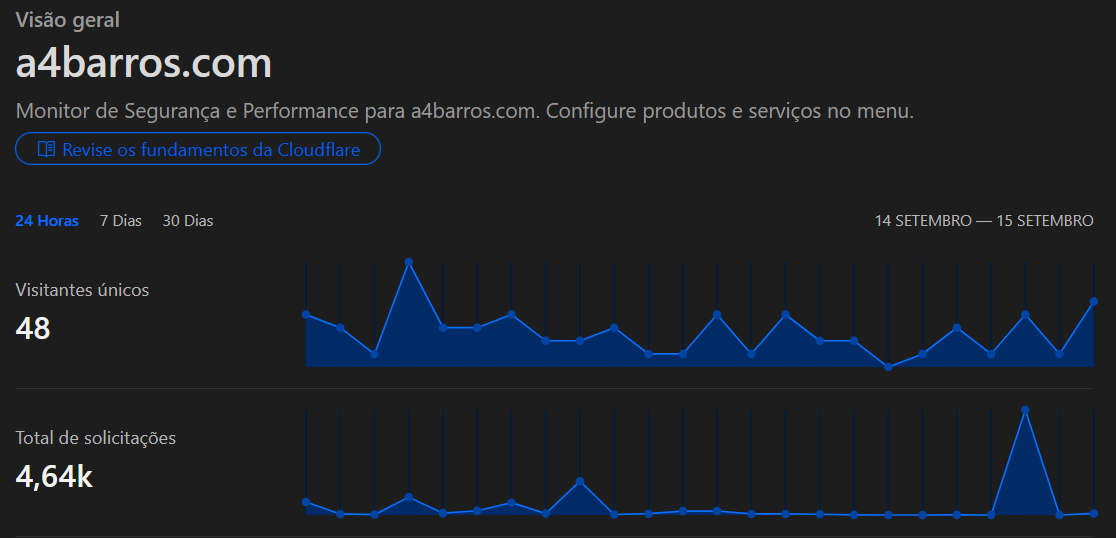
\includegraphics[width=400pt]{img/cloudflare-stat.png.png}
    \caption{Informações de acesso disponiblizadas pela Cloudflare}
    \label{fig:cloudflare-stat.png}
    \end{center}
\end{figure}